\chapter{Конструкторская часть}


\section{Концептуальная модель компилятора в нотации IDEF0}

Для создания функциональной модели компилятора, отражающей его основные этапы, наиболее наглядно использовать нотацию IDEF0. На рисунке \ref{fig:idef0-0} приведена концептуальная модель компилятора. На рисунке \ref{fig:idef0-1} представлена детализированная концептуальная модель компилятора в нотации IDEF0.

\begin{figure}[h!]
	\begin{center}
		{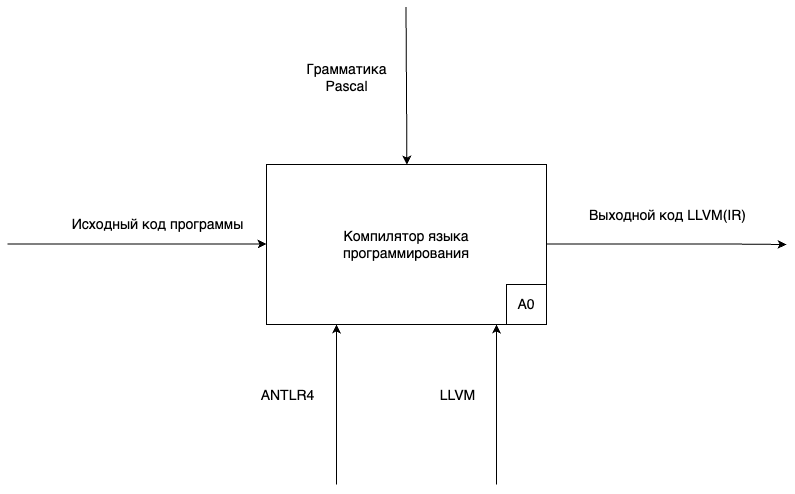
\includegraphics[scale = 0.5, angle=0]{../img/idef0/idef0-0.png}}
		\caption{Концептуальная модель компилятора в нотации IDEF0}
		\label{fig:idef0-0}
	\end{center}
\end{figure}


\begin{figure}[h!]
	\begin{center}
		{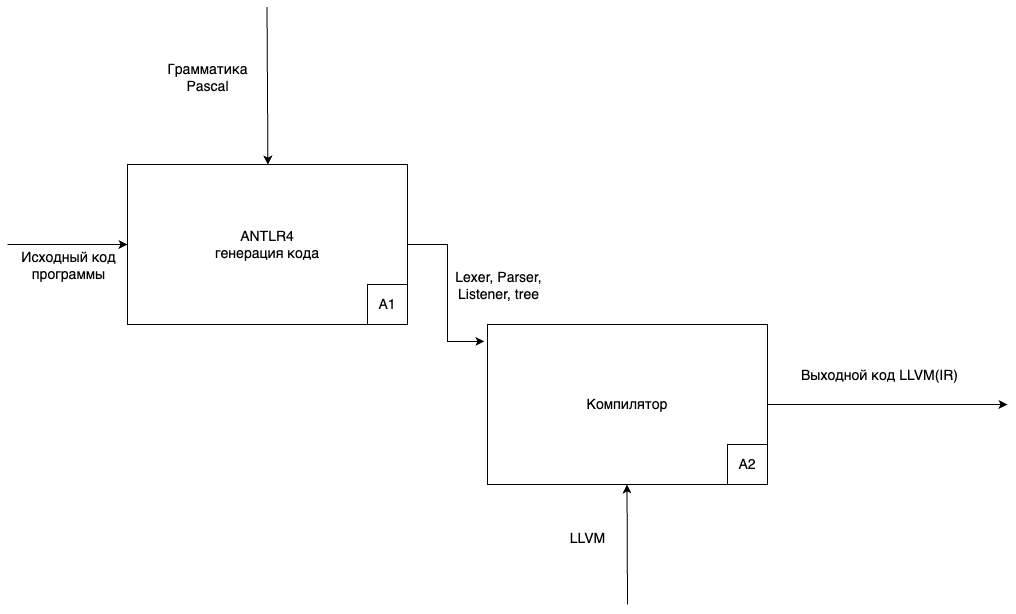
\includegraphics[scale = 0.4, angle=0]{../img/idef0/idef0-1.png}}
		\caption{Детализированная концептуальная модель компилятора в нотации IDEF0}
		\label{fig:idef0-1}
	\end{center}
\end{figure}

\clearpage


\section{Обход AST}

Обход абстрактного синтаксического дерева (AST) -- это ключевая операция в различных задачах компиляции и анализа программ, таких как интерпретация, оптимизация и трансформация кода. AST представляет собой иерархическую структуру, где узлы дерева соответствуют конструкциям исходного кода, а его ветви отражают синтаксическую структуру программы.

Для обхода абстрактного синтаксического дерева, созданного с помощью ANTLR, применяется паттерн слушателя. ANTLR автоматически генерирует интерфейс слушателя, который связан с встроенным классом, осуществляющим обход дерева. Слушатель предоставляет методы <<\texttt{enter}>> и <<\texttt{exit}>>, которые вызываются при входе и выходе из узлов дерева соответственно.

Интерфейс слушателя, создаваемый ANTLR, зависит от грамматики, заданной в проекте. Он включает методы <<\texttt{enter}>> и <<\texttt{exit}>> для каждого правила грамматики, которые необходимо реализовать в соответствии с требованиями проекта.


\section{Генерация выходного кода LLVM(IR)}

Чтобы создать код LLVM IR, нужно разработать алгоритм, который обходит каждую вершину дерева разбора, полученного с помощью парсера ANTLR, и генерирует соответствующий LLVM IR код в зависимости от типа этой вершины.

Общая схема алгоритма для генерации кода LLVM(IR) для компилятора, который умеет работать с цикалми, инициализацией и условными выражениями, приведена на рисунках \ref{fig:alg-1}-\ref{fig:alg-3}.

\begin{figure}[h!]
	\begin{center}
		{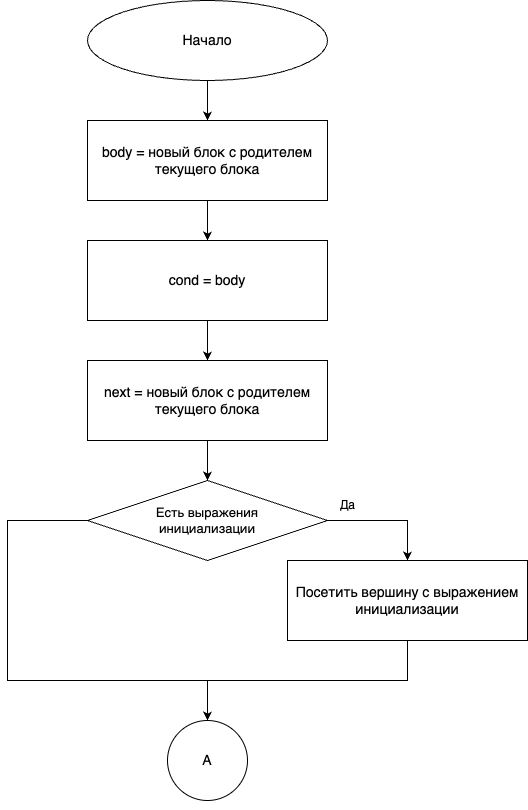
\includegraphics[scale = 0.5, angle=0]{../img/llvm/alg-1.png}}
		\caption{Схема алгоритма генерации LLVM(IR) (1)}
		\label{fig:alg-1}
	\end{center}
\end{figure}

\begin{figure}[h!]
	\begin{center}
		{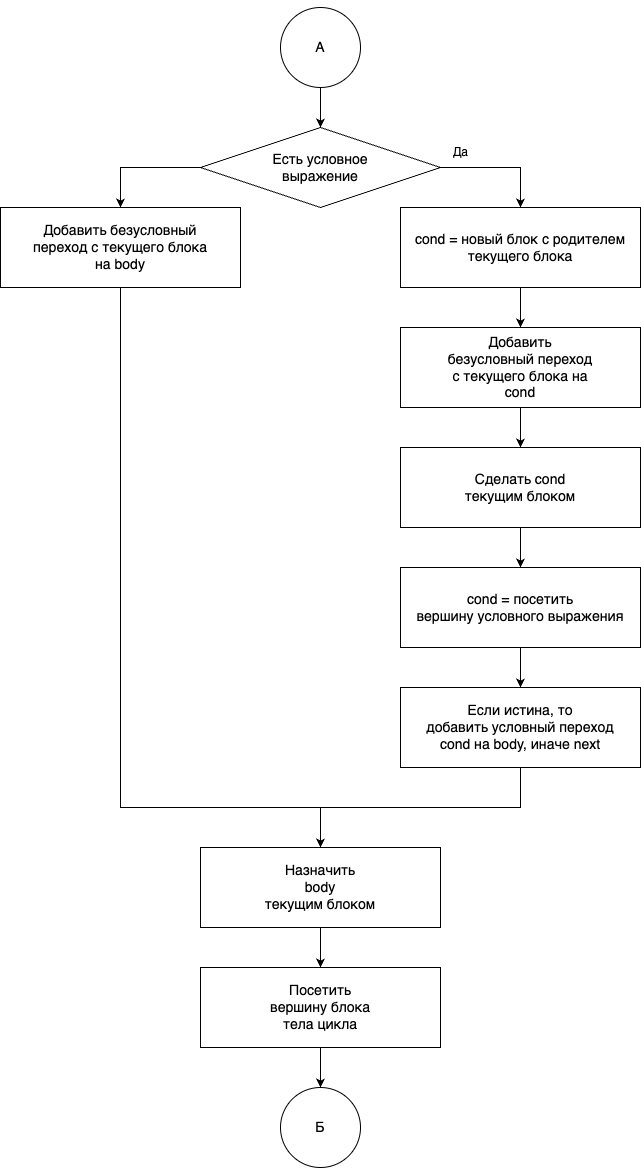
\includegraphics[scale = 0.5, angle=0]{../img/llvm/alg-2.png}}
		\caption{Схема алгоритма генерации LLVM(IR) (2)}
		\label{fig:alg-2}
	\end{center}
\end{figure}

\begin{figure}[h!]
	\begin{center}
		{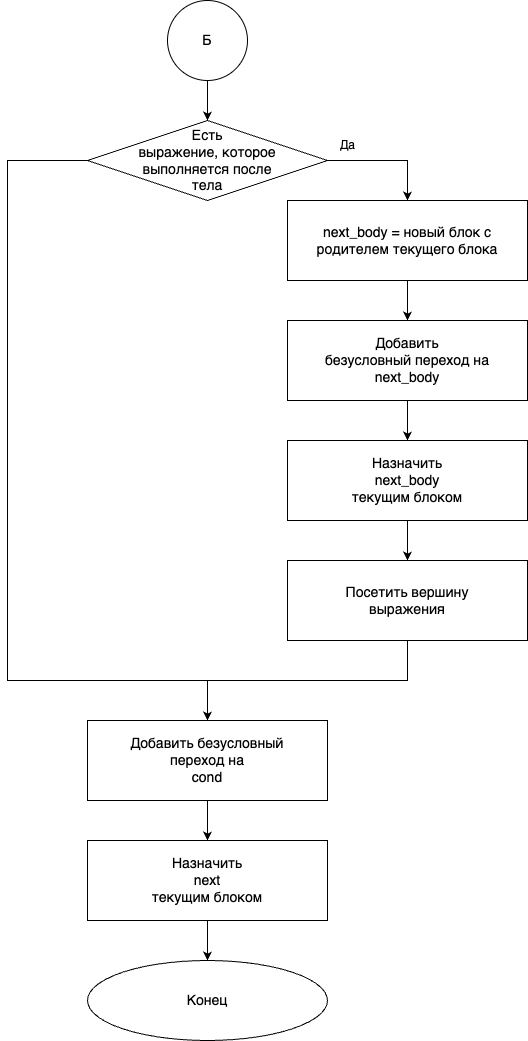
\includegraphics[scale = 0.5, angle=0]{../img/llvm/alg-3.png}}
		\caption{Схема алгоритма генерации LLVM(IR) (3)}
		\label{fig:alg-3}
	\end{center}
\end{figure}
